% Options for packages loaded elsewhere
\PassOptionsToPackage{unicode}{hyperref}
\PassOptionsToPackage{hyphens}{url}
\PassOptionsToPackage{dvipsnames,svgnames,x11names}{xcolor}
%
\documentclass[
  letterpaper,
  DIV=11,
  numbers=noendperiod]{scrartcl}

\usepackage{amsmath,amssymb}
\usepackage{iftex}
\ifPDFTeX
  \usepackage[T1]{fontenc}
  \usepackage[utf8]{inputenc}
  \usepackage{textcomp} % provide euro and other symbols
\else % if luatex or xetex
  \usepackage{unicode-math}
  \defaultfontfeatures{Scale=MatchLowercase}
  \defaultfontfeatures[\rmfamily]{Ligatures=TeX,Scale=1}
\fi
\usepackage{lmodern}
\ifPDFTeX\else  
    % xetex/luatex font selection
\fi
% Use upquote if available, for straight quotes in verbatim environments
\IfFileExists{upquote.sty}{\usepackage{upquote}}{}
\IfFileExists{microtype.sty}{% use microtype if available
  \usepackage[]{microtype}
  \UseMicrotypeSet[protrusion]{basicmath} % disable protrusion for tt fonts
}{}
\makeatletter
\@ifundefined{KOMAClassName}{% if non-KOMA class
  \IfFileExists{parskip.sty}{%
    \usepackage{parskip}
  }{% else
    \setlength{\parindent}{0pt}
    \setlength{\parskip}{6pt plus 2pt minus 1pt}}
}{% if KOMA class
  \KOMAoptions{parskip=half}}
\makeatother
\usepackage{xcolor}
\usepackage[left=2cm, right=2cm, top=2cm, bottom=2cm]{geometry}
\usepackage{soul}
\setlength{\emergencystretch}{3em} % prevent overfull lines
\setcounter{secnumdepth}{5}
% Make \paragraph and \subparagraph free-standing
\ifx\paragraph\undefined\else
  \let\oldparagraph\paragraph
  \renewcommand{\paragraph}[1]{\oldparagraph{#1}\mbox{}}
\fi
\ifx\subparagraph\undefined\else
  \let\oldsubparagraph\subparagraph
  \renewcommand{\subparagraph}[1]{\oldsubparagraph{#1}\mbox{}}
\fi

\usepackage{color}
\usepackage{fancyvrb}
\newcommand{\VerbBar}{|}
\newcommand{\VERB}{\Verb[commandchars=\\\{\}]}
\DefineVerbatimEnvironment{Highlighting}{Verbatim}{commandchars=\\\{\}}
% Add ',fontsize=\small' for more characters per line
\usepackage{framed}
\definecolor{shadecolor}{RGB}{241,243,245}
\newenvironment{Shaded}{\begin{snugshade}}{\end{snugshade}}
\newcommand{\AlertTok}[1]{\textcolor[rgb]{0.68,0.00,0.00}{#1}}
\newcommand{\AnnotationTok}[1]{\textcolor[rgb]{0.37,0.37,0.37}{#1}}
\newcommand{\AttributeTok}[1]{\textcolor[rgb]{0.40,0.45,0.13}{#1}}
\newcommand{\BaseNTok}[1]{\textcolor[rgb]{0.68,0.00,0.00}{#1}}
\newcommand{\BuiltInTok}[1]{\textcolor[rgb]{0.00,0.23,0.31}{#1}}
\newcommand{\CharTok}[1]{\textcolor[rgb]{0.13,0.47,0.30}{#1}}
\newcommand{\CommentTok}[1]{\textcolor[rgb]{0.37,0.37,0.37}{#1}}
\newcommand{\CommentVarTok}[1]{\textcolor[rgb]{0.37,0.37,0.37}{\textit{#1}}}
\newcommand{\ConstantTok}[1]{\textcolor[rgb]{0.56,0.35,0.01}{#1}}
\newcommand{\ControlFlowTok}[1]{\textcolor[rgb]{0.00,0.23,0.31}{#1}}
\newcommand{\DataTypeTok}[1]{\textcolor[rgb]{0.68,0.00,0.00}{#1}}
\newcommand{\DecValTok}[1]{\textcolor[rgb]{0.68,0.00,0.00}{#1}}
\newcommand{\DocumentationTok}[1]{\textcolor[rgb]{0.37,0.37,0.37}{\textit{#1}}}
\newcommand{\ErrorTok}[1]{\textcolor[rgb]{0.68,0.00,0.00}{#1}}
\newcommand{\ExtensionTok}[1]{\textcolor[rgb]{0.00,0.23,0.31}{#1}}
\newcommand{\FloatTok}[1]{\textcolor[rgb]{0.68,0.00,0.00}{#1}}
\newcommand{\FunctionTok}[1]{\textcolor[rgb]{0.28,0.35,0.67}{#1}}
\newcommand{\ImportTok}[1]{\textcolor[rgb]{0.00,0.46,0.62}{#1}}
\newcommand{\InformationTok}[1]{\textcolor[rgb]{0.37,0.37,0.37}{#1}}
\newcommand{\KeywordTok}[1]{\textcolor[rgb]{0.00,0.23,0.31}{#1}}
\newcommand{\NormalTok}[1]{\textcolor[rgb]{0.00,0.23,0.31}{#1}}
\newcommand{\OperatorTok}[1]{\textcolor[rgb]{0.37,0.37,0.37}{#1}}
\newcommand{\OtherTok}[1]{\textcolor[rgb]{0.00,0.23,0.31}{#1}}
\newcommand{\PreprocessorTok}[1]{\textcolor[rgb]{0.68,0.00,0.00}{#1}}
\newcommand{\RegionMarkerTok}[1]{\textcolor[rgb]{0.00,0.23,0.31}{#1}}
\newcommand{\SpecialCharTok}[1]{\textcolor[rgb]{0.37,0.37,0.37}{#1}}
\newcommand{\SpecialStringTok}[1]{\textcolor[rgb]{0.13,0.47,0.30}{#1}}
\newcommand{\StringTok}[1]{\textcolor[rgb]{0.13,0.47,0.30}{#1}}
\newcommand{\VariableTok}[1]{\textcolor[rgb]{0.07,0.07,0.07}{#1}}
\newcommand{\VerbatimStringTok}[1]{\textcolor[rgb]{0.13,0.47,0.30}{#1}}
\newcommand{\WarningTok}[1]{\textcolor[rgb]{0.37,0.37,0.37}{\textit{#1}}}

\providecommand{\tightlist}{%
  \setlength{\itemsep}{0pt}\setlength{\parskip}{0pt}}\usepackage{longtable,booktabs,array}
\usepackage{calc} % for calculating minipage widths
% Correct order of tables after \paragraph or \subparagraph
\usepackage{etoolbox}
\makeatletter
\patchcmd\longtable{\par}{\if@noskipsec\mbox{}\fi\par}{}{}
\makeatother
% Allow footnotes in longtable head/foot
\IfFileExists{footnotehyper.sty}{\usepackage{footnotehyper}}{\usepackage{footnote}}
\makesavenoteenv{longtable}
\usepackage{graphicx}
\makeatletter
\def\maxwidth{\ifdim\Gin@nat@width>\linewidth\linewidth\else\Gin@nat@width\fi}
\def\maxheight{\ifdim\Gin@nat@height>\textheight\textheight\else\Gin@nat@height\fi}
\makeatother
% Scale images if necessary, so that they will not overflow the page
% margins by default, and it is still possible to overwrite the defaults
% using explicit options in \includegraphics[width, height, ...]{}
\setkeys{Gin}{width=\maxwidth,height=\maxheight,keepaspectratio}
% Set default figure placement to htbp
\makeatletter
\def\fps@figure{htbp}
\makeatother

\usepackage{booktabs}
\usepackage{caption}
\usepackage{longtable}
\usepackage{colortbl}
\usepackage{array}
\KOMAoption{captions}{tableheading}
\makeatletter
\makeatother
\makeatletter
\makeatother
\makeatletter
\@ifpackageloaded{caption}{}{\usepackage{caption}}
\AtBeginDocument{%
\ifdefined\contentsname
  \renewcommand*\contentsname{Table of contents}
\else
  \newcommand\contentsname{Table of contents}
\fi
\ifdefined\listfigurename
  \renewcommand*\listfigurename{List of Figures}
\else
  \newcommand\listfigurename{List of Figures}
\fi
\ifdefined\listtablename
  \renewcommand*\listtablename{List of Tables}
\else
  \newcommand\listtablename{List of Tables}
\fi
\ifdefined\figurename
  \renewcommand*\figurename{Figure}
\else
  \newcommand\figurename{Figure}
\fi
\ifdefined\tablename
  \renewcommand*\tablename{Table}
\else
  \newcommand\tablename{Table}
\fi
}
\@ifpackageloaded{float}{}{\usepackage{float}}
\floatstyle{ruled}
\@ifundefined{c@chapter}{\newfloat{codelisting}{h}{lop}}{\newfloat{codelisting}{h}{lop}[chapter]}
\floatname{codelisting}{Listing}
\newcommand*\listoflistings{\listof{codelisting}{List of Listings}}
\makeatother
\makeatletter
\@ifpackageloaded{caption}{}{\usepackage{caption}}
\@ifpackageloaded{subcaption}{}{\usepackage{subcaption}}
\makeatother
\makeatletter
\@ifpackageloaded{tcolorbox}{}{\usepackage[skins,breakable]{tcolorbox}}
\makeatother
\makeatletter
\@ifundefined{shadecolor}{\definecolor{shadecolor}{rgb}{.97, .97, .97}}
\makeatother
\makeatletter
\makeatother
\makeatletter
\makeatother
\ifLuaTeX
  \usepackage{selnolig}  % disable illegal ligatures
\fi
\IfFileExists{bookmark.sty}{\usepackage{bookmark}}{\usepackage{hyperref}}
\IfFileExists{xurl.sty}{\usepackage{xurl}}{} % add URL line breaks if available
\urlstyle{same} % disable monospaced font for URLs
\hypersetup{
  pdftitle={Analysis of IMDB data set},
  pdfauthor={Group\_06},
  colorlinks=true,
  linkcolor={blue},
  filecolor={Maroon},
  citecolor={Blue},
  urlcolor={Blue},
  pdfcreator={LaTeX via pandoc}}

\title{Analysis of IMDB data set}
\author{Group\_06}
\date{}

\begin{document}
\maketitle
\ifdefined\Shaded\renewenvironment{Shaded}{\begin{tcolorbox}[interior hidden, boxrule=0pt, borderline west={3pt}{0pt}{shadecolor}, breakable, frame hidden, enhanced, sharp corners]}{\end{tcolorbox}}\fi

\hypertarget{sec-Intro}{%
\section{Introduction}\label{sec-Intro}}

The study aims to investigate the relationship between various film
attributes and IMDB ratings, drawing data from the IMDB film database
allocated. The data set comprises of the factors such as film ID,
release year, duration, budget, votes, genre, and IMDB rating. The
research question focuses on examining the factors that impact IMDB
ratings, particularly whether specific film properties contribute to
ratings greater than seven. A Generalized Linear Model (GLM) analysis is
conducted to derive the relationships between these properties and IMDB
ratings.

\hypertarget{sec-DW}{%
\section{Data Wrangling Methods}\label{sec-DW}}

Before we begin the analysis of our data, let's transform the data using
various tools. The process below describes the detailed data wrangling
techniques that are used to get the desired data set. After having a
glimpse of the data set, the `genre' column is converted to a type
factor type.

A check for missing values is conducted and it is found that 103
observations are missing from the column `length'. Missing values are
imputed with the median since median is a robust measure, less impacted
by outliers as much as mean. The function \emph{median( )} reveals the
median to be 90 minutes. However, it is observed in
Table~\ref{tbl-median-length} that the median lengths vary across the
different genres. With this information, the missing lengths of films
are replaced by median length of the respective genre.

\hypertarget{tbl-median-length}{}
\begin{longtable}[]{@{}lr@{}}
\caption{\label{tbl-median-length}Median length by
genre.}\tabularnewline
\toprule\noalign{}
genre & median\_length \\
\midrule\noalign{}
\endfirsthead
\toprule\noalign{}
genre & median\_length \\
\midrule\noalign{}
\endhead
\bottomrule\noalign{}
\endlastfoot
Action & 90.0 \\
Animation & 7.0 \\
Comedy & 91.0 \\
Documentary & 73.0 \\
Drama & 96.0 \\
Romance & 92.5 \\
Short & 13.5 \\
\end{longtable}

As per the research question, a new column `high\_rating' containing
binary variables corresponding to `rating' values is created. This
column takes a value of 1 for IMDB ratings greater than or equal to
seven and 0 for IMDB ratings less than seven. Additionally, another
categorical variable `rate' conveying the same is also added.

\hypertarget{sec-EDA}{%
\section{Exploratory Data Analysis}\label{sec-EDA}}

\hypertarget{view-the-data}{%
\subsection{View the data}\label{view-the-data}}

The data set has 1937 rows and 9 columns, 7 of which are from the
original data.

Let's have a look at the first five rows of the data frame.

\hypertarget{tbl-glimpse-dataset}{}
\begin{longtable}{rrrrrcrcc}
\caption{\label{tbl-glimpse-dataset}Glimpse of the first five rows in the IMDB data set. }\tabularnewline

\toprule
film\_id & year & length & budget & votes & genre & rating & high\_rating & rate \\ 
\midrule\addlinespace[2.5pt]
31804 & 2002 & 18 & 9.6 & 15 & Drama & 8.0 & 1 & Rating greater than 7 \\ 
25453 & 2000 & 98 & 13.8 & 23 & Action & 3.3 & 0 & Rating less than 7 \\ 
5479 & 1989 & 81 & 11.5 & 57 & Documentary & 7.9 & 1 & Rating greater than 7 \\ 
44235 & 1995 & 100 & 7.5 & 32 & Action & 3.4 & 0 & Rating less than 7 \\ 
14580 & 2003 & 80 & 10.8 & 30 & Action & 2.6 & 0 & Rating less than 7 \\ 
\bottomrule
\end{longtable}

The variables in Table~\ref{tbl-glimpse-dataset} are defined as:

\begin{itemize}
\item
  \textbf{film.id} : The unique identifier for the film
\item
  \textbf{year} : Year of release of the film in cinemas
\item
  \textbf{length} : Duration (in minutes)
\item
  \textbf{budget} : Budget for the films production (in \$1000000s)
\item
  \textbf{votes} : Number of positive votes received by viewers
\item
  \textbf{genre} : Genre of the film
\item
  \textbf{rating} :IMDB rating from 0 to 10
\item
  \textbf{high\_rating} : 1 for IMDB ratings greater than or equal to
  seven and 0 for ratings less than 7
\item
  \textbf{rate} : `Rating greater than 7' got high\_rating = 1 and
  `Rating less than 7' for high\_rating = 0 \clearpage
\end{itemize}

\hypertarget{sec-sum}{%
\subsection{Summary Statistics}\label{sec-sum}}

\hypertarget{tbl-summary-statistics}{}
\begin{longtable}{lrrrrrrr}
\caption{\label{tbl-summary-statistics}Summary statistics on the IMDB data by variables. }\tabularnewline

\toprule
Variables & Mean & Median & Std. Dev & Min & Max & IQR & Sample Size \\ 
\midrule\addlinespace[2.5pt]
year & $1,976.21$ & $1,982.00$ & $23.44$ & $1,896.00$ & $2,005.00$ & $39.00$ & $1,937.00$ \\ 
length & $82.88$ & $90.00$ & $35.62$ & $1.00$ & $316.00$ & $24.00$ & $1,937.00$ \\ 
budget & $12.03$ & $12.00$ & $2.92$ & $3.20$ & $21.20$ & $3.90$ & $1,937.00$ \\ 
votes & $590.47$ & $31.00$ & $3,894.33$ & $5.00$ & $103,854.00$ & $104.00$ & $1,937.00$ \\ 
rating & $5.29$ & $4.60$ & $2.05$ & $0.60$ & $9.30$ & $4.00$ & $1,937.00$ \\ 
\bottomrule
\end{longtable}

The Table~\ref{tbl-summary-statistics} shows that the summary for the
columns year, length, budget, votes and rating.

• For the variable year, the years of the films ranges from 1896 to
2005.

• For the variable length, the films runs from 1 minute to 316
minutes.The median for length of films is 90 minutes.

• For variable budget, the budget of films is from 3.2 (\$1000000s) to
21.2 (\$1000000s).The median budget of a film is 12(\$1000000s).

• For variable votes, the votes of films ranges from 5 to 103,854 which
suggests large variation. It can be observed the IQR is relatively large
as well.

\clearpage

\hypertarget{sec-cor}{%
\subsection{Correlation}\label{sec-cor}}

\begin{figure}

{\centering 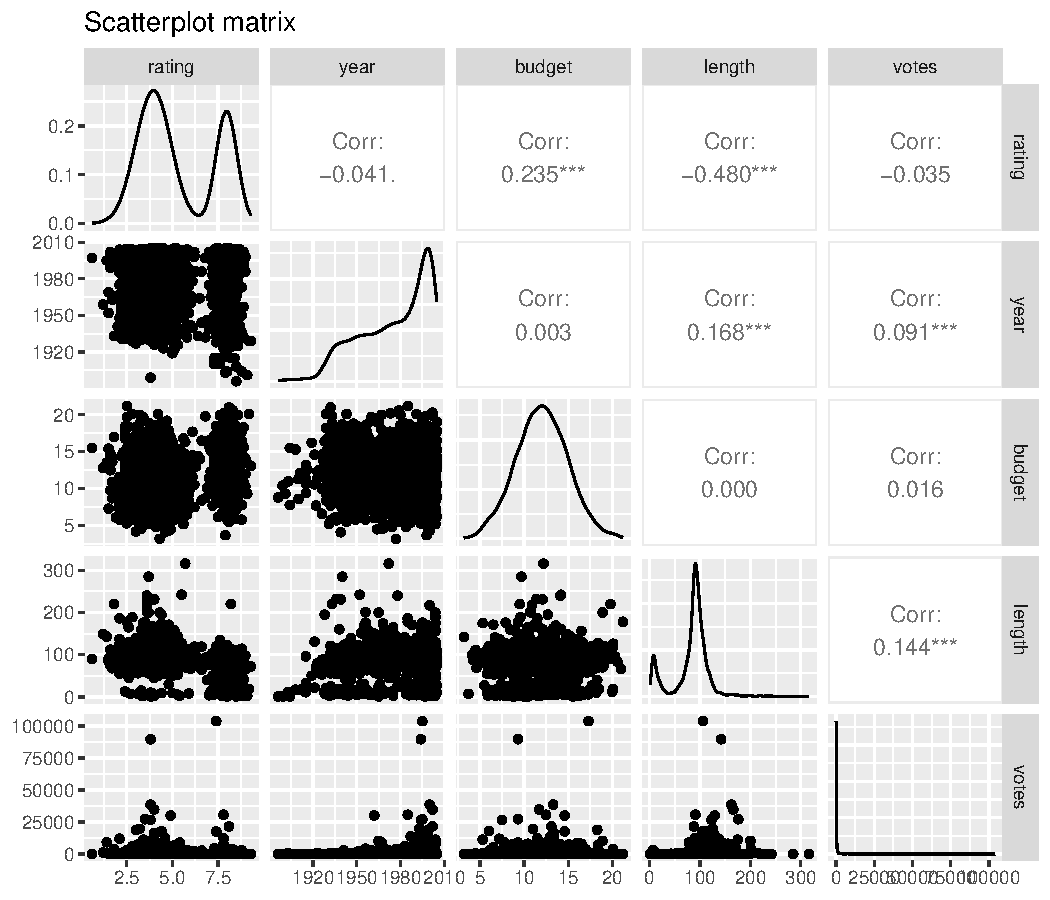
\includegraphics{Group_06_Analysis_files/figure-pdf/fig-scatterplot-matrix-1.pdf}

}

\caption{\label{fig-scatterplot-matrix}Scatterplot matrix between rating
and explanatory variables.}

\end{figure}

The Figure~\ref{fig-scatterplot-matrix} shows weak correlation between
the variables. `length' shows not so strong negative correlation with
'rating.

\hypertarget{sec-viz}{%
\subsection{Visualization}\label{sec-viz}}

\hypertarget{histograms}{%
\subsubsection{Histograms}\label{histograms}}

\begin{figure}

{\centering 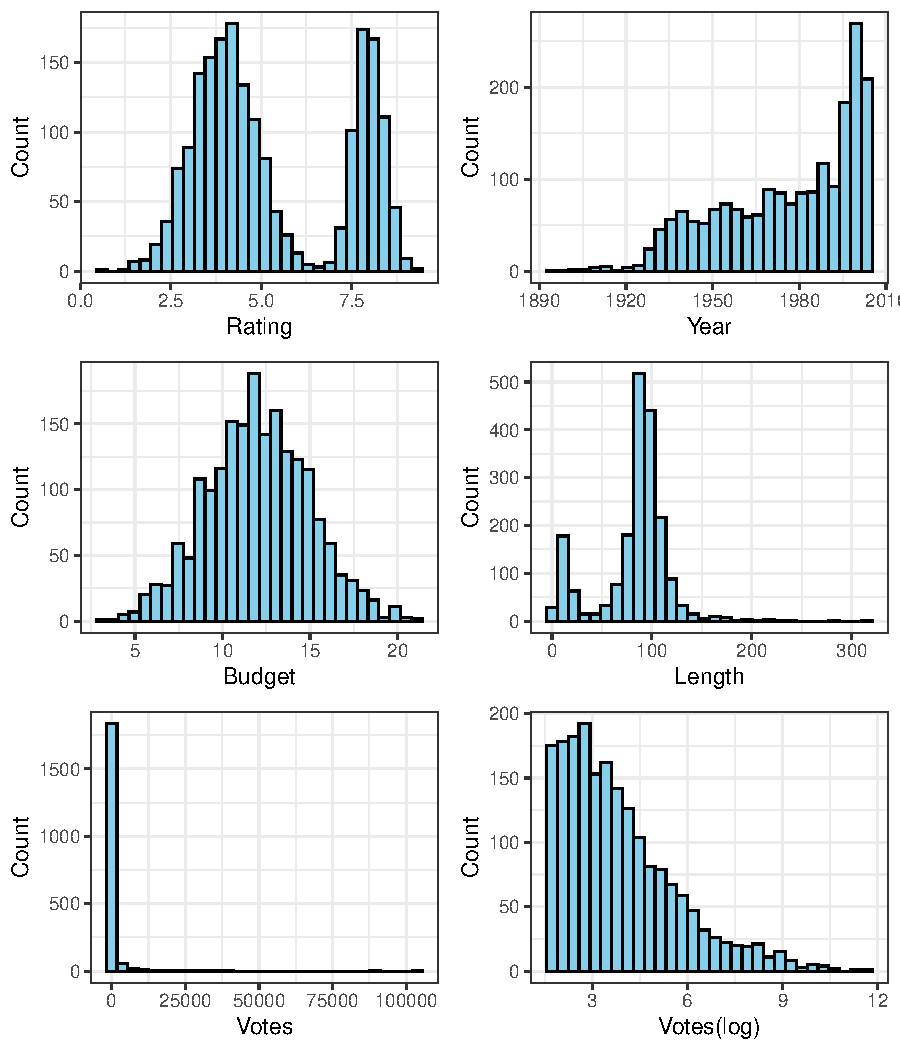
\includegraphics{Group_06_Analysis_files/figure-pdf/fig-histograms-1.pdf}

}

\caption{\label{fig-histograms}Histograms of statistical distribution
for varibles}

\end{figure}

The Figure~\ref{fig-histograms} shows that the data structures follow
exponential distributions. The variable `votes' displays skewness due to
large difference in values of maximum and minimum values. To reduce this
skewness and facilitate more robust analysis, a logarithmic
transformation is used.

\clearpage

\hypertarget{scatter-plot-for-rating-vs-explanatory-variables}{%
\subsubsection{Scatter plot for rating vs explanatory
variables}\label{scatter-plot-for-rating-vs-explanatory-variables}}

The Figure~\ref{fig-scatterplots-relationship} suggests that there seems
to be no linear relationship between the response variable and the
explanatory variables which justifies the weak correlation observed
earlier.

\begin{figure}

{\centering 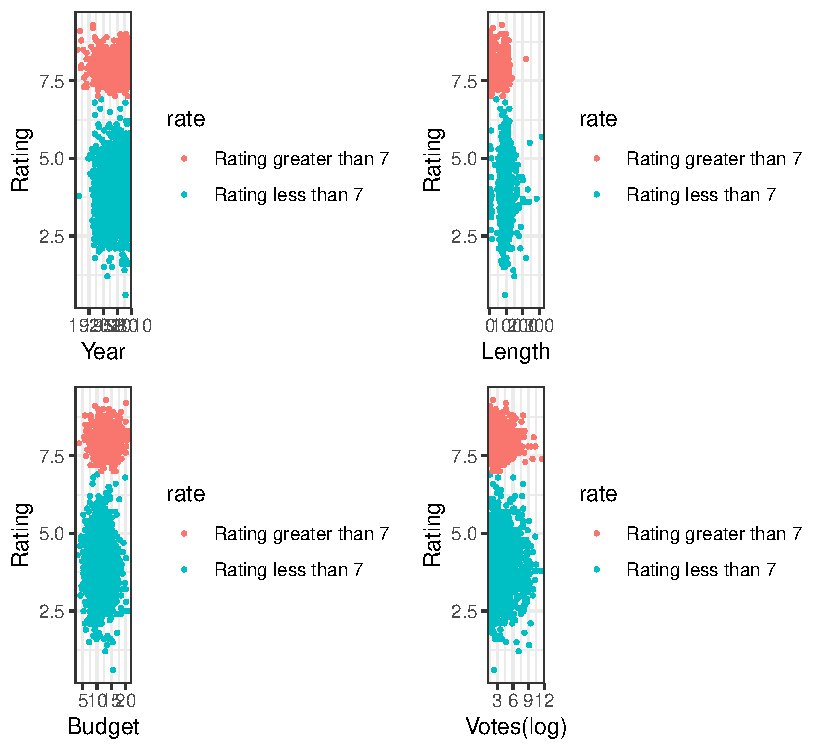
\includegraphics{Group_06_Analysis_files/figure-pdf/fig-scatterplots-relationship-1.pdf}

}

\caption{\label{fig-scatterplots-relationship}Scatterplots between
rating and four explanatory variables.}

\end{figure}

\clearpage

\hypertarget{boxplot-for-genre}{%
\subsubsection{Boxplot for genre}\label{boxplot-for-genre}}

\begin{figure}

{\centering 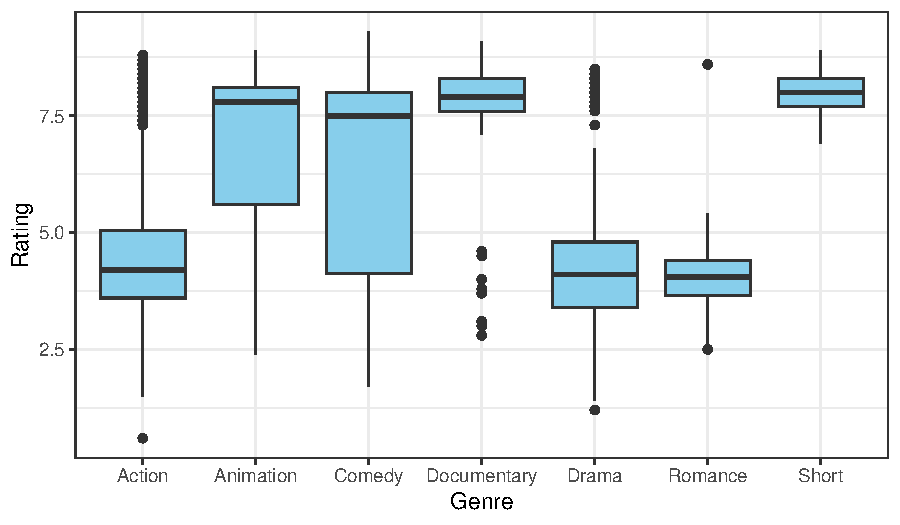
\includegraphics{Group_06_Analysis_files/figure-pdf/fig-boxplot-ratings-1.pdf}

}

\caption{\label{fig-boxplot-ratings}Boxplot of ratings by genre.}

\end{figure}

The Figure~\ref{fig-boxplot-ratings} distribution of rating genre wise.
Outliers for ratings can be seen for the genre's Action, Documentary,
Drama and Romance. \clearpage

\hypertarget{the-relationship-response-and-explanatory-variable}{%
\subsection{The relationship response and explanatory
variable}\label{the-relationship-response-and-explanatory-variable}}

\hypertarget{variable-1-length}{%
\subsubsection{Variable 1: Length}\label{variable-1-length}}

\begin{figure}

{\centering 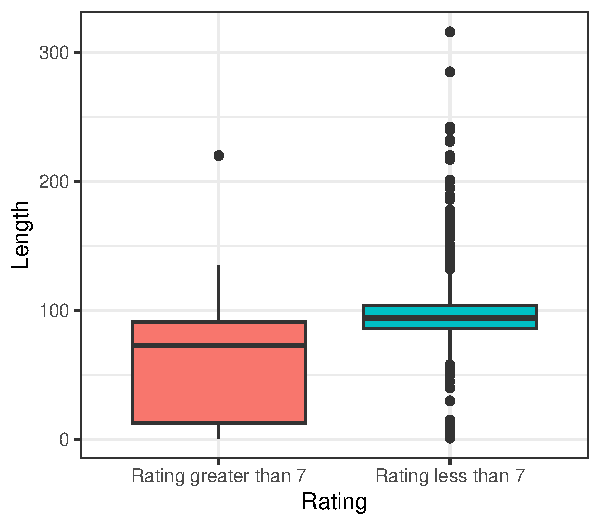
\includegraphics{Group_06_Analysis_files/figure-pdf/fig-boxplot-length-1.pdf}

}

\caption{\label{fig-boxplot-length}Boxplot of length by rating.}

\end{figure}

The Figure~\ref{fig-boxplot-length} shows that the median film length of
films with `Rating greater than 7' is less than that of `Rating less
than 7' films. It can be observed IQR of `Rating less than 7' is smaller
but has many outliers.

\hypertarget{tbl-summary-length}{}
\begin{longtable}{crrrrrrr}
\caption{\label{tbl-summary-length}Summary statistics on length by rating. }\tabularnewline

\toprule
rate & Mean & Median & St.Dev & Min & Max & IQR & Sample Size \\ 
\midrule\addlinespace[2.5pt]
Rating greater than 7 & $57.05$ & $73.00$ & $39.49$ & $1.00$ & $220.00$ & $78.25$ & $644.00$ \\ 
Rating less than 7 & $95.74$ & $94.00$ & $25.03$ & $1.00$ & $316.00$ & $18.00$ & $1,293.00$ \\ 
\bottomrule
\end{longtable}

The Table~\ref{tbl-summary-length} The median length film with `Rating
greater than 7' is (73 minutes) lower than that with `Rating less than
7' (95.74 minutes).

\clearpage

\hypertarget{variable-2-budget}{%
\subsubsection{Variable 2 : budget}\label{variable-2-budget}}

\begin{figure}

{\centering 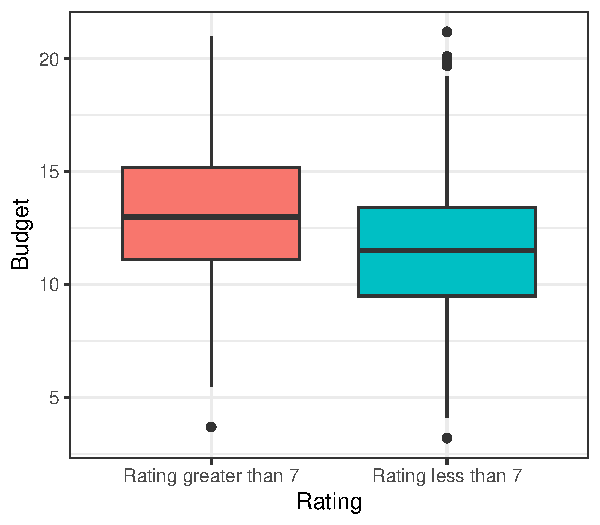
\includegraphics{Group_06_Analysis_files/figure-pdf/fig-boxplot-budget-1.pdf}

}

\caption{\label{fig-boxplot-budget}Boxplot of budget by rating.}

\end{figure}

The Figure~\ref{fig-boxplot-budget} shows that the median budget film of
`Rating greater than 7' is slightly higher than that of `Rating less
than 7' films. There are 9 outliers.

\hypertarget{tbl-summary-budget}{}
\begin{longtable}{crrrrrrr}
\caption{\label{tbl-summary-budget}Summary statistics on budget by rating. }\tabularnewline

\toprule
rate & Mean & Median & Std. Dev & Min & Max & IQR & Sample Size \\ 
\midrule\addlinespace[2.5pt]
Rating greater than 7 & $13.09$ & $13.00$ & $2.84$ & $3.70$ & $21.00$ & $4.10$ & $644.00$ \\ 
Rating less than 7 & $11.51$ & $11.50$ & $2.82$ & $3.20$ & $21.20$ & $3.90$ & $1,293.00$ \\ 
\bottomrule
\end{longtable}

The Table~\ref{tbl-summary-budget} shows that the mean and median for
`Rating greater than 7' is almost equal. Similarly, it can be observed
for and `Rating less than 7' as well. This suggests a normal
distribution. The variability is also equivalent for the 2 categories.

\clearpage

\hypertarget{variable-3-log_votes}{%
\subsubsection{Variable 3 : log\_votes}\label{variable-3-log_votes}}

\begin{figure}

{\centering 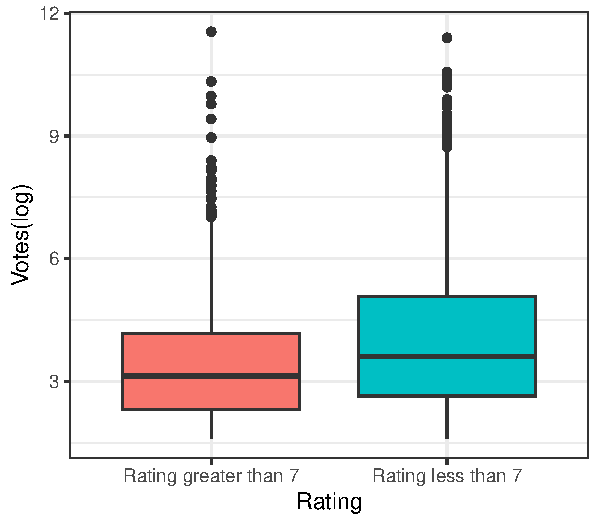
\includegraphics{Group_06_Analysis_files/figure-pdf/fig-boxplot-logvotes-1.pdf}

}

\caption{\label{fig-boxplot-logvotes}Boxplot of log\_votes by rating.}

\end{figure}

The Figure~\ref{fig-boxplot-logvotes} shows that the median log\_votes
film of `Rating greater than 7' films is lower than that of `Rating less
than 7' films.

\hypertarget{tbl-summary-logvotes}{}
\begin{longtable}{crrrrrrr}
\caption{\label{tbl-summary-logvotes}Summary statistics of votes(log) by rating. }\tabularnewline

\toprule
rate & Mean & Median & Std. Dev & Min & Max & IQR & Sample Size \\ 
\midrule\addlinespace[2.5pt]
Rating greater than 7 & $3.47$ & $3.14$ & $1.58$ & $1.61$ & $11.55$ & $1.88$ & $644.00$ \\ 
Rating less than 7 & $4.03$ & $3.61$ & $1.86$ & $1.61$ & $11.40$ & $2.43$ & $1,293.00$ \\ 
\bottomrule
\end{longtable}

The Table~\ref{tbl-summary-logvotes} shows that the mean and median for
`Rating greater than 7' is almost equal.

\clearpage

\hypertarget{variable-4-genre}{%
\subsubsection{Variable 4 : genre}\label{variable-4-genre}}

The ratio of ratings above 7 to ratings below 7 and sample sizes for
each type

\hypertarget{tbl-summary-genre}{}
\begin{longtable}{crrc}
\caption{\label{tbl-summary-genre}Summary statistics of genre }\tabularnewline

\toprule
genre & Rating greater than 7 & Rating less than 7 & genre\_sum\_count \\ 
\midrule\addlinespace[2.5pt]
Action & 15.9\%  (92) & 84.1\% (487) & 579 \\ 
Animation & 73.5\%  (86) & 26.5\%  (31) & 117 \\ 
Comedy & 59.1\% (266) & 40.9\% (184) & 450 \\ 
Documentary & 89.9\%  (89) & 10.1\%  (10) & 99 \\ 
Drama & 5.7\%  (34) & 94.3\% (561) & 595 \\ 
Romance & 5.0\%   (1) & 95.0\%  (19) & 20 \\ 
Short & 98.7\%  (76) & 1.3\%   (1) & 77 \\ 
\bottomrule
\end{longtable}

It can be seen the size for the genre `Romance' is only 20, which is
comparatively small. We observe the following: - Animation, Documentary,
Short - have more films with `Rating greater than 7' - Action, Drama,
Romance - have more films with `Rating less than 7' - Comedy - films
with `Rating greater than 7' are moderately higher than `Rating less
than 7'

\begin{figure}

{\centering 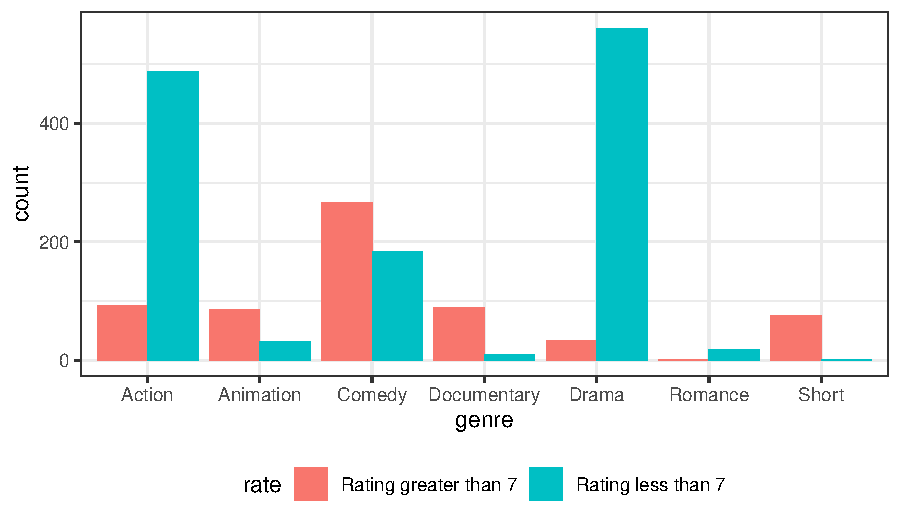
\includegraphics{Group_06_Analysis_files/figure-pdf/fig-dodgedbarplot-genre-1.pdf}

}

\caption{\label{fig-dodgedbarplot-genre}Dodged barplot of genre by
rating.}

\end{figure}

The Figure~\ref{fig-dodgedbarplot-genre} displays the information in the
table Table~\ref{tbl-summary-genre}

\clearpage

\hypertarget{outliers}{%
\subsubsection{Outliers}\label{outliers}}

It can be observed from the scatter plot that there are outliers present
especially for length and votes. Then extreme outlier values are
replaced by threshold values corresponding to specific percentiles -

\begin{itemize}
\item
  length - 10th and 90th percentiles
\item
  budget- 5th percentile and 95th percentile
\item
  log\_votes- Since logarithmic transformation had already removed a
  considerable amount of outlier, the threshold was set to 10th and 90th
  percentiles
\end{itemize}

This replacement strategy aims to mitigate the impact of outliers on the
analysis while retaining the overall distribution of the data. The
approach ensures that extreme values are transformed to less extreme
values, thereby improving the robustness of subsequent statistical
analyses.

\hypertarget{sec-Formal}{%
\section{Formal Data Analysis}\label{sec-Formal}}

The response variable `high\_rating' is the rating for 1937 films taking
the values 1 for `Rating greater than 7' and 0 for `Rating less than 7'.
Predictors include the properties of films `year', `length', `budget',
`log\_votes' and `genre'. It is assumed that
\(high\_rating_i \sim \text{Bin}(1, p_i)\) where
\emph{p\textsubscript{i}} is the probability of film with `Rating
greater than 7' for the \emph{i}th film. A logistic regression model is
fitted.

\hypertarget{sec-fm}{%
\subsection{Fitting the Model}\label{sec-fm}}

Baseline category for our binary response high\_rating is 0 i.e `Rating
less than 7'

\hypertarget{sec-sat.model}{%
\subsubsection{Saturated Model}\label{sec-sat.model}}

A full model with all the continuous independent variables `year',
`length', `budget', `log\_votes' and categorical explanatory variable
`genre' is explored:

\[\begin{aligned}\ln\left(\frac{p_i}{1-p_i}\right) &= \alpha + \beta_1 \cdot \textrm{year}_i + \beta_2 \cdot \textrm{length}_i + \beta_3 \cdot \textrm{budget}_i  + \beta_4 \cdot \textrm{log_votes}_i \\&\quad + \beta_{\textrm{Animation}} \cdot \mathbb{I}_{\textrm{Animation}}(i) + \beta_{\textrm{Comedy}} \cdot \mathbb{I}_{\textrm{Comedy}}(i) \\&\quad + \beta_{\textrm{Document}} \cdot \mathbb{I}_{\textrm{Document}}(i) + \beta_{\textrm{Drama}} \cdot \mathbb{I}_{\textrm{Drama}}(i) \\&\quad + \beta_{\textrm{Romance}} \cdot \mathbb{I}_{\textrm{Romance}}(i) + \beta_{\textrm{Short}} \cdot \mathbb{I}_{\textrm{Short}}(i)\end{aligned}\]

\[\mathbb{I}_{\textrm{genre}}(i) = \begin{cases}
1 & \textrm{if } i\textrm{th observation is in genre}, \\
0 & \textrm{otherwise}.
\end{cases}\]

\[\textrm{genre} = \{\textrm{Animation, Comedy, Documentary, Drama, Romance, Short}\}\]
\clearpage

\hypertarget{tbl-m0_model-Summary}{}
\begin{longtable}{lrrrrrr}
\caption{\label{tbl-m0_model-Summary}Summary for Saturated Model }\tabularnewline

\toprule
term & estimate & std.error & statistic & p.value & 2.5 \% & 97.5 \% \\ 
\midrule\addlinespace[2.5pt]
(Intercept) & -21.841 & 7.289 & -2.996 & 0.003 & -36.239 & -7.641 \\ 
year & 0.009 & 0.004 & 2.548 & 0.011 & 0.002 & 0.017 \\ 
length & -0.070 & 0.005 & -13.995 & 0.000 & -0.080 & -0.061 \\ 
budget & 0.560 & 0.039 & 14.357 & 0.000 & 0.485 & 0.638 \\ 
log\_votes & 0.019 & 0.063 & 0.306 & 0.760 & -0.104 & 0.142 \\ 
genreAnimation & -0.425 & 0.413 & -1.028 & 0.304 & -1.241 & 0.382 \\ 
genreComedy & 3.079 & 0.217 & 14.170 & 0.000 & 2.663 & 3.515 \\ 
genreDocumentary & 5.064 & 0.460 & 11.012 & 0.000 & 4.204 & 6.015 \\ 
genreDrama & -1.631 & 0.279 & -5.844 & 0.000 & -2.198 & -1.101 \\ 
genreRomance & -2.433 & 1.854 & -1.312 & 0.189 & -6.270 & 0.323 \\ 
genreShort & 3.226 & 1.072 & 3.010 & 0.003 & 1.521 & 6.160 \\ 
\bottomrule
\end{longtable}

Baseline category for explanatory variable `genre' is ``Action''

From Table~\ref{tbl-m0_model-Summary} the following can be observed:

\begin{itemize}
\item
  \textbf{Variable Selection} log\_votes has a p-value of 0.760. This
  suggests that there this parameter should not be included in the
  model.
\item
  \textbf{Hypothesis Testing} Since log-votes has p-value \textgreater{}
  0.05, it is not statistically significant and does not contribute in
  explaining the variation in the response variable.
\item
  \textbf{95\% Confidence Interval} The approximate 95\% confidence
  interval of log\_votes contains zero, it can be concluded log\_votes
  is not statistically significant.
\end{itemize}

\textbf{Analysis of Deviance Table}

\hypertarget{tbl-dev}{}
\begin{longtable}{rrrr}
\caption{\label{tbl-dev}Anova Table }\tabularnewline

\toprule
Df & Deviance & Resid. Df & Resid. Dev \\ 
\midrule\addlinespace[2.5pt]
NA & NA & $1,936.00$ & $2,463.54$ \\ 
$1.00$ & $3.01$ & $1,935.00$ & $2,460.53$ \\ 
$1.00$ & $588.93$ & $1,934.00$ & $1,871.60$ \\ 
$1.00$ & $189.57$ & $1,933.00$ & $1,682.03$ \\ 
$1.00$ & $3.20$ & $1,932.00$ & $1,678.83$ \\ 
$6.00$ & $660.86$ & $1,926.00$ & $1,017.97$ \\ 
\bottomrule
\end{longtable}

In Table~\ref{tbl-dev} each row represents a term (predictor variable)
added to the model. It can be observed that largest reduction in
residual deviance comes when adding `genre' and the smallest when adding
`year' and `log\_votes'. A model without `year' and `log\_votes' could
be tried. \clearpage

\textbf{Goodness-of-fit}

\begin{enumerate}
\def\labelenumi{\arabic{enumi}.}
\item
  \ul{Deviance} : for a GLM model that fits the data well the
  approximate deviance D is \(\chi^2(m-p)\) where \emph{m} is the number
  of parameters in the saturated model (full model) and \emph{p} is the
  number of parameters in the model of interest. In the above model,
  2463.5-1018.0 is larger than 95th percentile of the
  \(\chi^2(1936-1926)\) . There is no evidence of lack of fit.
\item
  \ul{Hosmer-Lemeshow goodness of fit test}: For a model with binary
  responses,

  H\textsubscript{0} = the model fits the data well,

  H\textsubscript{1} = the model does not fit the data well
\end{enumerate}

\begin{Shaded}
\begin{Highlighting}[]
\CommentTok{\#Deviance\#}
\NormalTok{m0\_q1 }\OtherTok{\textless{}{-}} \FunctionTok{qchisq}\NormalTok{(}\AttributeTok{df=}\DecValTok{10}\NormalTok{, }\AttributeTok{p=}\FloatTok{0.95}\NormalTok{) }\CommentTok{\# 18.30704}
\CommentTok{\# Hosmer{-}Lemeshow goodness of fit test}
\NormalTok{m0\_hl }\OtherTok{\textless{}{-}} \FunctionTok{HLTest}\NormalTok{(m0\_model, }\AttributeTok{g =} \DecValTok{6}\NormalTok{)}
\end{Highlighting}
\end{Shaded}

A large p-value indicates no lack of fit. From the above output there is
no evidence of lack of fit.

\textbf{Assumptions}

\begin{enumerate}
\def\labelenumi{\arabic{enumi}.}
\item
  The dependent variable is binary
\item
  Independence of observations
\item
  The independent variable do not correlate too strongly with each other
\item
  Linearity of continuous explanatory variables and the log-odds outcome
\item
  No outliers
\end{enumerate}

The first assumption is fulfilled as the the 'rating; has been converted
to a binary variable in accordance. For asuumption 2, since the
observation belong to independent fils, it is satisfied. For assumption
3, Figure~\ref{fig-scatterplot-matrix} justifies that there are no
strong correlations between the independent variables.
\clearpage Assumption 4: Check linearity of continuous variables against
log odds of the dependent variable

\begin{figure}

{\centering 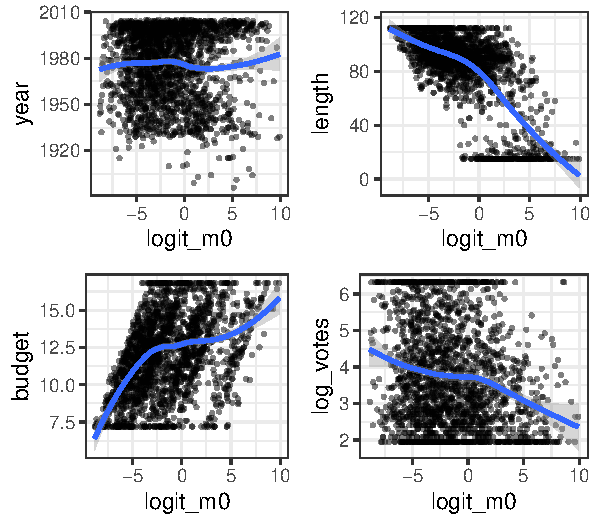
\includegraphics{Group_06_Analysis_files/figure-pdf/fig-lin-m0-1.pdf}

}

\caption{\label{fig-lin-m0}Checking Linearity for m0\_model}

\end{figure}

The relationship between continuous variables against log-odds seems to
be fairly linear. \clearpage Assumption 5: Checking for outliers

\begin{figure}

{\centering 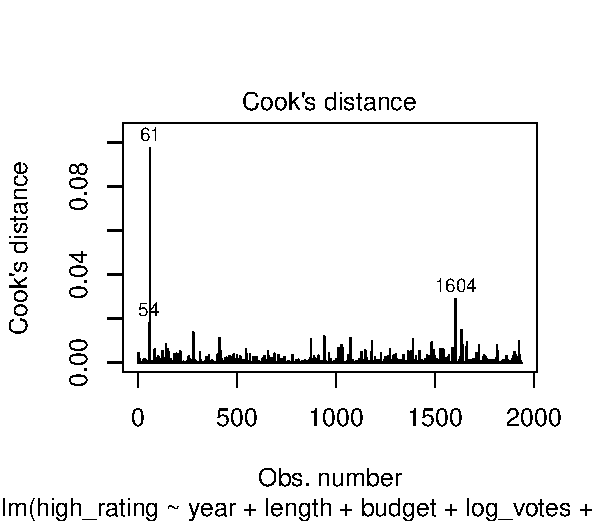
\includegraphics{Group_06_Analysis_files/figure-pdf/fig-cook-m0-1.pdf}

}

\caption{\label{fig-cook-m0}Checking Outliers for m0\_model}

\end{figure}

The model has outliers which can be observed in Figure~\ref{fig-cook-m0}
.This is due to the outliers present in the data set.

\hypertarget{sec-m1.model}{%
\subsubsection{Model 1}\label{sec-m1.model}}

A model with continuous independent variables with `year', `length',
`budget' and categorical explanatory variable is explored:

\[\begin{aligned}\ln\left(\frac{p_i}{1-p_i}\right) &= \alpha + \beta_1 \cdot \textrm{year}_i + \beta_2 \cdot \textrm{length}_i + \beta_3 \cdot \textrm{budget}_i \\&\quad + \beta_{\textrm{Animation}} \cdot \mathbb{I}_{\textrm{Animation}}(i) + \beta_{\textrm{Comedy}} \cdot \mathbb{I}_{\textrm{Comedy}}(i) \\&\quad + \beta_{\textrm{Document}} \cdot \mathbb{I}_{\textrm{Document}}(i) + \beta_{\textrm{Drama}} \cdot \mathbb{I}_{\textrm{Drama}}(i) \\&\quad + \beta_{\textrm{Romance}} \cdot \mathbb{I}_{\textrm{Romance}}(i) + \beta_{\textrm{Short}} \cdot \mathbb{I}_{\textrm{Short}}(i)\end{aligned}\]

\[\mathbb{I}_{\textrm{genre}}(i) = \begin{cases}
1 & \textrm{if } i\textrm{th observation is in genre}, \\
0 & \textrm{otherwise}.
\end{cases}\]

\[\textrm{genre} = \{\textrm{Animation, Comedy, Documentary, Drama, Romance, Short}\}\]
\clearpage

\hypertarget{tbl-m1_model-Summary}{}
\begin{longtable}{lrrrrrr}
\caption{\label{tbl-m1_model-Summary}Summary for m1\_model }\tabularnewline

\toprule
term & estimate & std.error & statistic & p.value & 2.5 \% & 97.5 \% \\ 
\midrule\addlinespace[2.5pt]
(Intercept) & -22.196 & 7.194 & -3.085 & 0.002 & -36.415 & -8.190 \\ 
year & 0.010 & 0.004 & 2.645 & 0.008 & 0.003 & 0.017 \\ 
length & -0.070 & 0.005 & -14.259 & 0.000 & -0.080 & -0.061 \\ 
budget & 0.559 & 0.039 & 14.355 & 0.000 & 0.485 & 0.638 \\ 
genreAnimation & -0.407 & 0.409 & -0.995 & 0.320 & -1.215 & 0.391 \\ 
genreComedy & 3.090 & 0.214 & 14.413 & 0.000 & 2.679 & 3.521 \\ 
genreDocumentary & 5.054 & 0.459 & 11.019 & 0.000 & 4.197 & 6.003 \\ 
genreDrama & -1.629 & 0.279 & -5.842 & 0.000 & -2.196 & -1.100 \\ 
genreRomance & -2.414 & 1.846 & -1.308 & 0.191 & -6.240 & 0.334 \\ 
genreShort & 3.226 & 1.072 & 3.010 & 0.003 & 1.521 & 6.159 \\ 
\bottomrule
\end{longtable}

From Table~\ref{tbl-m1_model-Summary} the following can be observed:

\begin{itemize}
\item
  \textbf{Variable Selection} All the estimates are statistically
  significant with a p-value \textless{} 0.05.
\item
  \textbf{Hypothesis Testing} Since p-values \textgreater{} 0.05 for all
  the parameters, the predictors are statistically significant and
  contributes to explaining the variation in the response variable.
\item
  \textbf{95\% Confidence Interval} The approximate 95\% confidence
  interval for all the parameters do not contain 0, it can be concluded
  they are statistically significant.
\end{itemize}

\textbf{Goodness-of-fit}

\begin{enumerate}
\def\labelenumi{\arabic{enumi}.}
\item
  \ul{Deviance} : In the above model, 2463.5-1018.1 = 1445.4 is larger
  than 95th percentile of the \(\chi^2(1936-1927)\) = 16.92 . There is
  no evidence of lack of fit.
\item
  \ul{Hosmer-Lemeshow goodness of fit test}: From the output, there is
  no evidence of lack of fit.
\end{enumerate}

\begin{Shaded}
\begin{Highlighting}[]
\CommentTok{\#Deviance\#}
\NormalTok{m1\_q }\OtherTok{\textless{}{-}} \FunctionTok{qchisq}\NormalTok{(}\AttributeTok{df=}\DecValTok{9}\NormalTok{, }\AttributeTok{p=}\FloatTok{0.95}\NormalTok{) }\CommentTok{\# 16.91898}
\CommentTok{\#Hosmer{-}Lemeshow goodness of fit test\#}
\NormalTok{m1\_hl }\OtherTok{\textless{}{-}} \FunctionTok{HLTest}\NormalTok{(m1\_model, }\AttributeTok{g =} \DecValTok{6}\NormalTok{) }\CommentTok{\#p{-}value = 0.1181 \textgreater{}0.05}
\end{Highlighting}
\end{Shaded}

\textbf{Assumptions}

\begin{enumerate}
\def\labelenumi{\arabic{enumi}.}
\item
  The dependent variable is binary
\item
  Independence of observations
\item
  The independent variable do not correlate too strongly with each other
\item
  Linearity of continuous explanatory variables and the log-odds outcome
\item
  No outliers
\end{enumerate}

The first assumption is fulfilled as the the 'rating; has been converted
to a binary variable in accordance. For assumption 2, since the
observation belong to independent films, it is satisfied. For assumption
3, Figure~\ref{fig-scatterplot-matrix} justifies that there are no
strong correlations between the independent variables.
\clearpage Assumption 4: Check linearity of continuous variables against
log odds of the dependent variable

\begin{figure}

{\centering 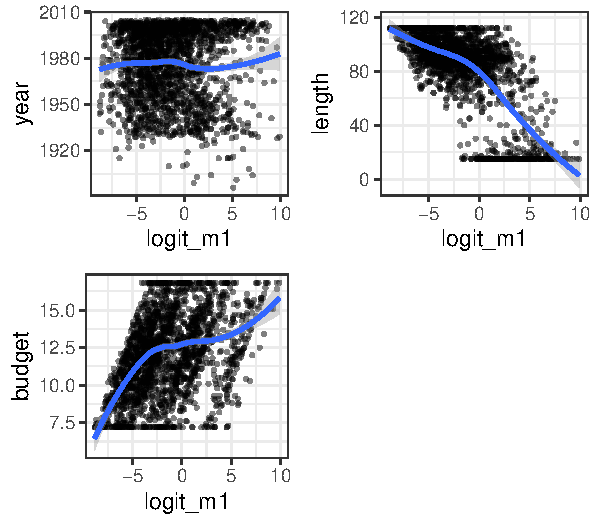
\includegraphics{Group_06_Analysis_files/figure-pdf/fig-lin-m1-1.pdf}

}

\caption{\label{fig-lin-m1}Checking Linearity for m1\_model}

\end{figure}

The relationship between continuous variables against log-odds seems to
be fairly linear for all the variables in Figure~\ref{fig-lin-m1}
\clearpage Assumption 5:Checking for outliers

\begin{figure}

{\centering 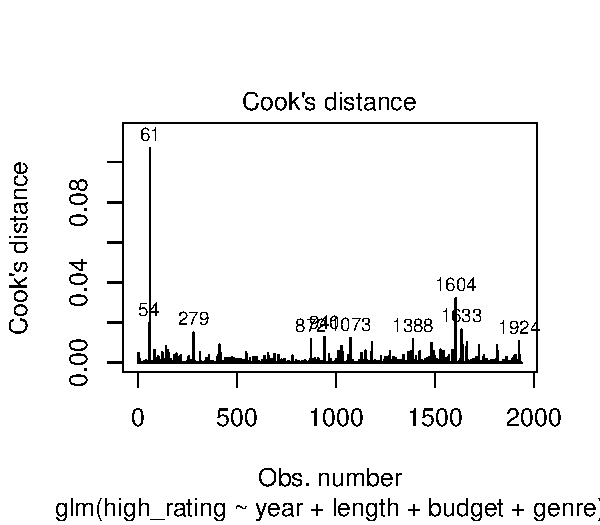
\includegraphics{Group_06_Analysis_files/figure-pdf/fig-cook-m1-1.pdf}

}

\caption{\label{fig-cook-m1}Checking Outliers for m1\_model}

\end{figure}

The model has outliers which can be observed in
Figure~\ref{fig-cook-m1}. This is due to the outliers present in the
data set.

\hypertarget{sec-m2.model}{%
\subsubsection{Model 2}\label{sec-m2.model}}

\[\begin{aligned}
\ln\left(\frac{p_i}{1-p_i}\right) &= \alpha + \beta_1 \cdot \textrm{length}_i + \beta_2 \cdot \textrm{budget}_i \\
&\quad + \beta_{\textrm{Animation}} \cdot \mathbb{I}_{\textrm{Animation}}(i) + \beta_{\textrm{Comedy}} \cdot \mathbb{I}_{\textrm{Comedy}}(i) \\
&\quad + \beta_{\textrm{Document}} \cdot \mathbb{I}_{\textrm{Document}}(i) + \beta_{\textrm{Drama}} \cdot \mathbb{I}_{\textrm{Drama}}(i) \\
&\quad + \beta_{\textrm{Romance}} \cdot \mathbb{I}_{\textrm{Romance}}(i) + \beta_{\textrm{Short}} \cdot \mathbb{I}_{\textrm{Short}}(i)
\end{aligned}\]

\[\mathbb{I}_{\textrm{genre}}(i) = \begin{cases}
1 & \textrm{if genre of } i\textrm{th observation is in genre}, \\
0 & \textrm{otherwise}.
\end{cases}\]

\[\textrm{genre} = \{\textrm{Animation, Comedy, Documentary, Drama, Romance, Short}\}\]
\clearpage

\hypertarget{tbl-m2_model-Summary}{}
\begin{longtable}{lrrrrrr}
\caption{\label{tbl-m2_model-Summary}Summary for m2\_model }\tabularnewline

\toprule
term & estimate & std.error & statistic & p.value & 2.5 \% & 97.5 \% \\ 
\midrule\addlinespace[2.5pt]
(Intercept) & -3.244 & 0.551 & -5.888 & 0.000 & -4.337 & -2.175 \\ 
length & -0.067 & 0.005 & -14.305 & 0.000 & -0.077 & -0.058 \\ 
budget & 0.554 & 0.039 & 14.363 & 0.000 & 0.480 & 0.632 \\ 
genreAnimation & -0.409 & 0.408 & -1.003 & 0.316 & -1.214 & 0.387 \\ 
genreComedy & 3.056 & 0.213 & 14.346 & 0.000 & 2.648 & 3.484 \\ 
genreDocumentary & 5.154 & 0.456 & 11.300 & 0.000 & 4.302 & 6.099 \\ 
genreDrama & -1.584 & 0.274 & -5.790 & 0.000 & -2.139 & -1.064 \\ 
genreRomance & -2.362 & 1.705 & -1.385 & 0.166 & -6.043 & 0.237 \\ 
genreShort & 3.428 & 1.069 & 3.206 & 0.001 & 1.730 & 6.359 \\ 
\bottomrule
\end{longtable}

From the Table~\ref{tbl-m2_model-Summary} following can be observed:

\begin{itemize}
\item
  \textbf{Variable Selection} All the estimates are statistically
  significant with a p-value \textless{} 0.05. However, it
  Table~\ref{tbl-dev} computed that the smallest reduction in residual
  deviance comes from `year'.
\item
  \textbf{Hypothesis Testing} Since p-values \textgreater{} 0.05 for all
  the parameters, the predictors are statistically significant and
  contributes to explaining the variation in the response variable.
\item
  \textbf{95\% Confidence Interval} The approximate 95\% confidence
  interval for all the parameters do not contain 0, it can be concluded
  they are statistically significant.
\end{itemize}

\textbf{Goodness-of-fit}

\begin{enumerate}
\def\labelenumi{\arabic{enumi}.}
\item
  \ul{Deviance} : In the above model, 2463.5-1025.2 = 1438.3 is larger
  than 95th percentile of the \(\chi^2(1936-1928)\) = 16.92 . There is
  no evidence of lack of fit.
\item
  \ul{Hosmer-Lemeshow goodness of fit test}: For a model with binary
  responses,

  H\textsubscript{0} = the model fits the data well,, H\textsubscript{1}
  = the model does not fit the data well
\end{enumerate}

\begin{Shaded}
\begin{Highlighting}[]
\CommentTok{\#Deviance\#}
\NormalTok{m2\_q }\OtherTok{\textless{}{-}} \FunctionTok{qchisq}\NormalTok{(}\AttributeTok{df=}\DecValTok{9}\NormalTok{, }\AttributeTok{p=}\FloatTok{0.95}\NormalTok{) }\CommentTok{\# 16.91898}
\CommentTok{\# Hosmer{-}Lemeshow goodness of fit test}
\NormalTok{m2\_hl }\OtherTok{\textless{}{-}} \FunctionTok{HLTest}\NormalTok{(m2\_model, }\AttributeTok{g =} \DecValTok{6}\NormalTok{) }\CommentTok{\# 0.3674}
\end{Highlighting}
\end{Shaded}

A large p-value indicates no lack of fit. From the above output there is
no evidence of lack of fit.

\textbf{Assumptions}

\begin{enumerate}
\def\labelenumi{\arabic{enumi}.}
\item
  The dependent variable is binary
\item
  Independence of observations
\item
  The independent variable do not correlate too strongly with each other
\item
  Linearity of continuous explanatory variables and the log-odds outcome
\item
  No outliers \clearpage The first assumption is fulfilled as the the
  'rating; has been converted to a binary variable in accordance. For
  assumption 2, since the observation belong to independent films, it is
  satisfied. For assumption 3, Figure~\ref{fig-scatterplot-matrix}
  justifies that there are no strong correlations between the
  independent variables.
\end{enumerate}

Assumption 4: Check linearity of continuous variables against log odds
of the dependent variable

\begin{figure}

{\centering 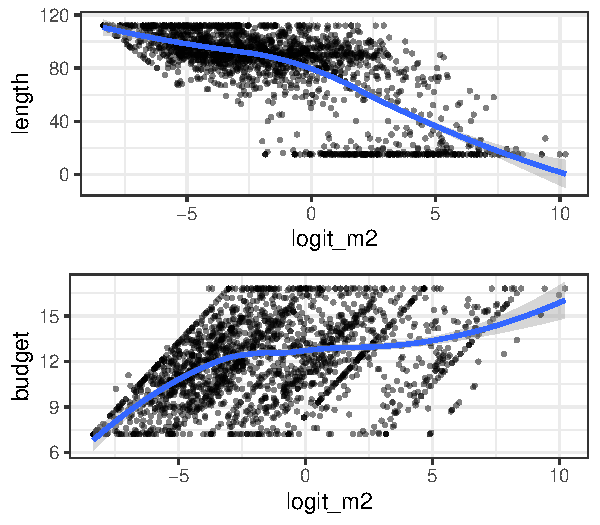
\includegraphics{Group_06_Analysis_files/figure-pdf/fig-lin-m2-1.pdf}

}

\caption{\label{fig-lin-m2}Checking Linearity for m2\_model}

\end{figure}

The relationship between continuous variables against log-odds seems to
be fairly linear for all the variables in Figure~\ref{fig-lin-m2}
\clearpage Assumption 5: Checking for outliers

\begin{figure}

{\centering 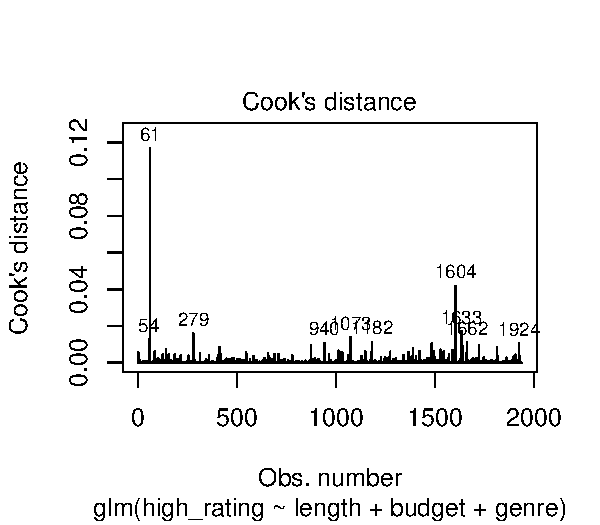
\includegraphics{Group_06_Analysis_files/figure-pdf/fig-cook-m2-1.pdf}

}

\caption{\label{fig-cook-m2}Checking Outliers for m2\_model}

\end{figure}

The model has outliers which can be observed in Figure~\ref{fig-cook-m2}
. This is due to the outliers present in the data set.

\hypertarget{Sec-lop}{%
\subsubsection{Log-Odds, Odds and Probabilities}\label{Sec-lop}}

\textbf{Log-Odds}

The baseline category for out binary response variables is `Rating less
than 7'. This implies from the logistic regression model are on the
log-odds scale for `Rating greater than 7' in comparison to the
baseline'. `Rating less than 7'.

The coefficients are extracted from the Table~\ref{tbl-m2_model-Summary}
and are found to be:

\begin{itemize}
\item
  \textbf{Intercept (-3.244):} This represents the log-odds of the
  outcome when all predictor variables are zero.
\item
  \textbf{Length (-0.067):} For every one-unit increase in the
  ``length'' variable, holding all other variables constant, the
  log-odds of the outcome \ul{decrease} by 0.067.
\item
  \textbf{Budget (0.554):} For every one-unit increase in the ``budget''
  variable, holding all other variables constant, the log-odds of the
  outcome increase by 0.554 .
\item
  \textbf{Genre Animation (-0.409):} Observations belonging to the
  ``Animation'' genre have log-odds 0.409 \ul{lower} than observations
  belonging to the ``Action'' genre, holding all other variables
  constant.
\item
  \textbf{Genre Comedy (3.056):} Observations belonging to the
  ``Comedy'' genre have log-odds 3.056 higher than observations
  belonging to the ``Action'' genre, holding all other variables
  constant.
\item
  \textbf{Genre Documentary (5.154):} Observations belonging to the
  ``Documentary'' genre have log-odds 5.154 higher than observations
  belonging to the ``Action'' genre, holding all other variables
  constant.
\item
  \textbf{Genre Drama (-1.584):} Observations belonging to the ``Drama''
  genre have log-odds 1.584 \ul{lower} than observations belonging to
  the ``Action'' genre, holding all other variables constant.
\item
  \textbf{Genre Romance (-2.362):} Observations belonging to the
  ``Romance'' genre have log-odds 2.362 \ul{lower} than observations
  belonging to the ``Action'' genre, holding all other variables
  constant.
\item
  \textbf{Genre Short (3.428):} Observations belonging to the ``Short''
  genre have log-odds 3.428 higher than observations belonging to the
  ``Action'' genre, holding all other variables constant.
\end{itemize}

The equation are as follows:

For the ``Action'' genre (reference category):

\[\ln\left(\frac{p_i}{1-p_i}\right) = -3.244 - 0.067 \times \textrm{length}_i + 0.554 \times \textrm{budget}_i\]

For the ``Animation'' genre:

\[\ln\left(\frac{p_i}{1-p_i}\right) = -3.244 - 0.067 \times \textrm{length}_i + 0.554 \times \textrm{budget}_i - 0.409\]

For the ``Comedy'' genre:

\[\ln\left(\frac{p_i}{1-p_i}\right) = -3.244 - 0.067 \times \textrm{length}_i + 0.554 \times \textrm{budget}_i + 3.056\]

For the ``Documentary'' genre:

\[\ln\left(\frac{p_i}{1-p_i}\right) = -3.244 - 0.067 \times \textrm{length}_i + 0.554 \times \textrm{budget}_i + 5.154\]

For the ``Drama'' genre:

\[\ln\left(\frac{p_i}{1-p_i}\right) = -3.244 - 0.067 \times \textrm{length}_i + 0.554 \times \textrm{budget}_i - 1.584\]

For the ``Romance'' genre:

\[\ln\left(\frac{p_i}{1-p_i}\right) = -3.244 - 0.067 \times \textrm{length}_i + 0.554 \times \textrm{budget}_i - 2.362\]

For the ``Short'' genre:

\[\ln\left(\frac{p_i}{1-p_i}\right) = -3.244 - 0.067 \times \textrm{length}_i + 0.554 \times \textrm{budget}_i + 3.428\]

where \emph{p =} Prob(Rating Greater than 7)

and \emph{1-p =} Prob(Rating less than 7)

95\% confidence interval for these log-odds can be found in
Table~\ref{tbl-m2_model-Summary}

Hence the point estimate for the log-odds can be displayed graphically
in Figure~\ref{fig-logodds} with there corresponding 95\% confidence
interval.

\begin{figure}

{\centering 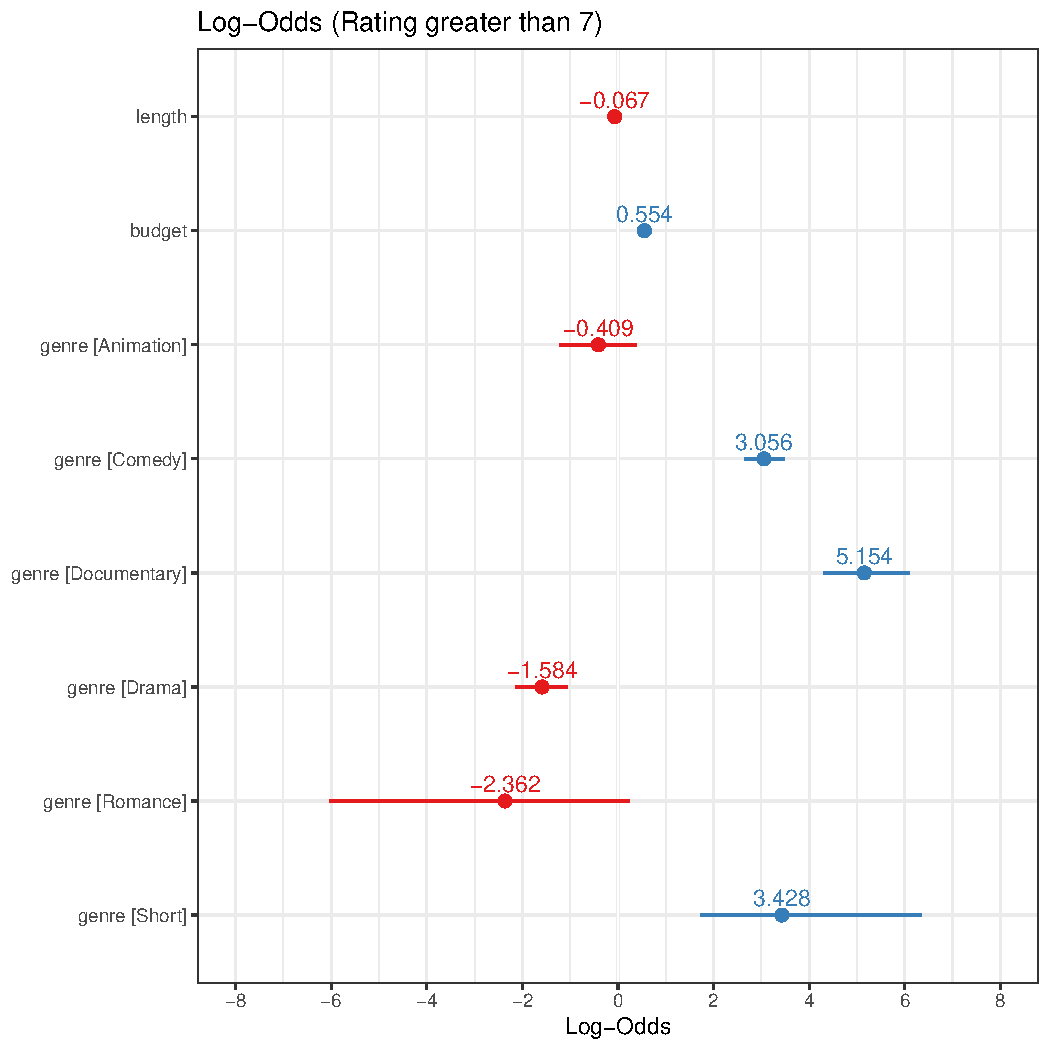
\includegraphics{Group_06_Analysis_files/figure-pdf/fig-logodds-1.pdf}

}

\caption{\label{fig-logodds}Plot for Log-Odds}

\end{figure}

\clearpage

The estimates of the log-odds were added to thr data set.

\textbf{Odds}

\[\begin{aligned}
\text{Odds}(p_i) &= \frac{p_i}{1 - p_i} \\
&= \exp\left(\alpha + \beta_1 \cdot \text{length}_i + \beta_2 \cdot \text{budget}_i \right. \\
&\quad + \beta_{\text{Animation}} \cdot \mathbb{I}_{\text{Animation}}(i) + \beta_{\text{Comedy}} \cdot \mathbb{I}_{\text{Comedy}}(i) \\
&\quad + \beta_{\text{Document}} \cdot \mathbb{I}_{\text{Document}}(i) + \beta_{\text{Drama}} \cdot \mathbb{I}_{\text{Drama}}(i) \\
&\quad + \left. \beta_{\text{Romance}} \cdot \mathbb{I}_{\text{Romance}}(i) + \beta_{\text{Short}} \cdot \mathbb{I}_{\text{Short}}(i)\right)
\end{aligned}\]

On the~\textbf{odds}~scale the regression coefficients are given by:

\hypertarget{tbl-odds-Summary}{}
\begin{longtable}{lr}
\caption{\label{tbl-odds-Summary}Odds Ratios for m2\_model }\tabularnewline

\toprule
Variable & Odds Ratio \\ 
\midrule\addlinespace[2.5pt]
(Intercept) & 0.039 \\ 
length & 0.935 \\ 
budget & 1.740 \\ 
genreAnimation & 0.664 \\ 
genreComedy & 21.234 \\ 
genreDocumentary & 173.181 \\ 
genreDrama & 0.205 \\ 
genreRomance & 0.094 \\ 
genreShort & 30.816 \\ 
\bottomrule
\end{longtable}

On the odds scale,

\begin{itemize}
\item
  The intercept coefficient (0.039) represents the odds of the film
  being in the ``high\_rating'' category when all predictor variables
  are zero. Given this is not viable, the intercept value is very close
  to zero.
\item
  For each one unit increase in ``length'', the odds of the film being
  in the ``high\_rating'' category decrease by a factor of approximately
  0.935.
\item
  For each one unit increase in ``budget'', the odds of the film being
  in the ``high\_rating'' category increase by a factor of approximately
  1.740.
\item
  For each film belonging to ``Animation'' genre, the odds of the film
  being in the ``high\_rating'' category approximately decrease by the
  factor 0.664 times the odds of the reference category (``Action'').
\item
  For each film belonging to ``Comedy'' genre, theodds of the film being
  in the ``high\_rating'' category approximately increase by the factor
  of 21.234 the odds of the reference category.
\item
  For each film belonging to ``Documentary'' genre, the odds of the film
  being in the ``high\_rating'' category approximately increase by the
  factor of 173.181 the odds of the reference category.
\item
  For each film belonging to ``Drama'' genre odds, the odds of the film
  being in the ``high\_rating'' category approximately decrease by the
  factor of 0.205 the odds of the reference category.
\item
  For each film belonging to ``Romance'' genre, the odds of the film
  being in the ``high\_rating'' category approximately decrease by the
  factor of 0.094 the odds of the reference category.
\item
  For each film belonging to ``Short'' genre, the odds of the film being
  in the ``high\_rating'' category approximately increase by the factor
  of 30.816 the odds of the reference category.
\end{itemize}

The 95\% confidence interval for the odds can be obtained by applying
exponential to the log odds interval:

\hypertarget{tbl-odds-CI}{}
\begin{longtable}{rr}
\caption{\label{tbl-odds-CI}Odds Ratios for m2\_model }\tabularnewline

\caption*{
{\large Odds Ratio Confidence Intervals}
} \\ 
\toprule
2.5 \% & 97.5 \% \\ 
\midrule\addlinespace[2.5pt]
0.013 & 0.114 \\ 
0.926 & 0.943 \\ 
1.617 & 1.881 \\ 
0.297 & 1.472 \\ 
14.123 & 32.574 \\ 
73.854 & 445.210 \\ 
0.118 & 0.345 \\ 
0.002 & 1.267 \\ 
5.643 & 577.912 \\ 
\bottomrule
\end{longtable}

Hence the point estimate for the odds can be displayed graphically in
Figure~\ref{fig-odds} with there corresponding 95\% confidence interval.
\clearpage

\begin{figure}

{\centering 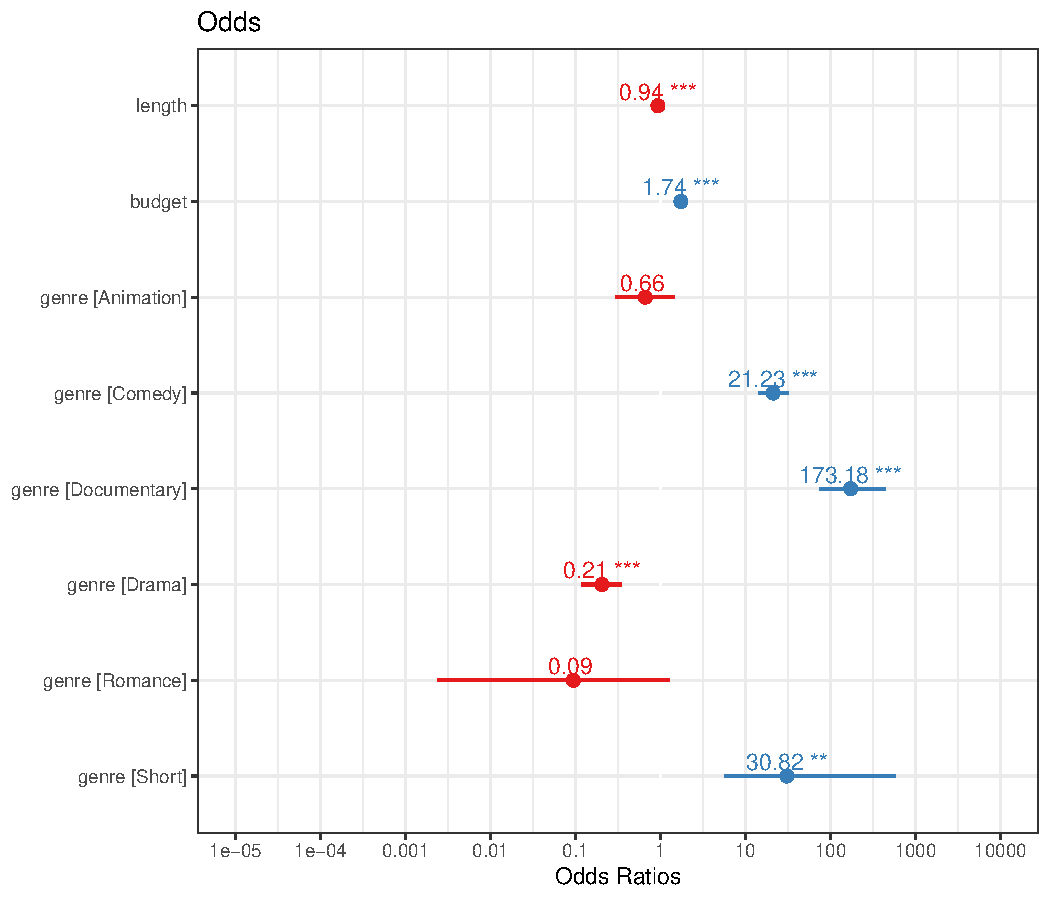
\includegraphics{Group_06_Analysis_files/figure-pdf/fig-odds-1.pdf}

}

\caption{\label{fig-odds}Plot for Odds}

\end{figure}

\clearpage

The odds estimates were added to the data set.

\textbf{Probabilities}

Probabilities added to the data set which have been formulated by using
the fitted() function

\[p = \frac{\text{odds}}{\text{odds} + 1}\]

The predicted probabilities of high rating against the films `length'
and `budget' by the films `genre' is shown in
Figure~\ref{fig-probabilities-plot} .

\begin{figure}

{\centering 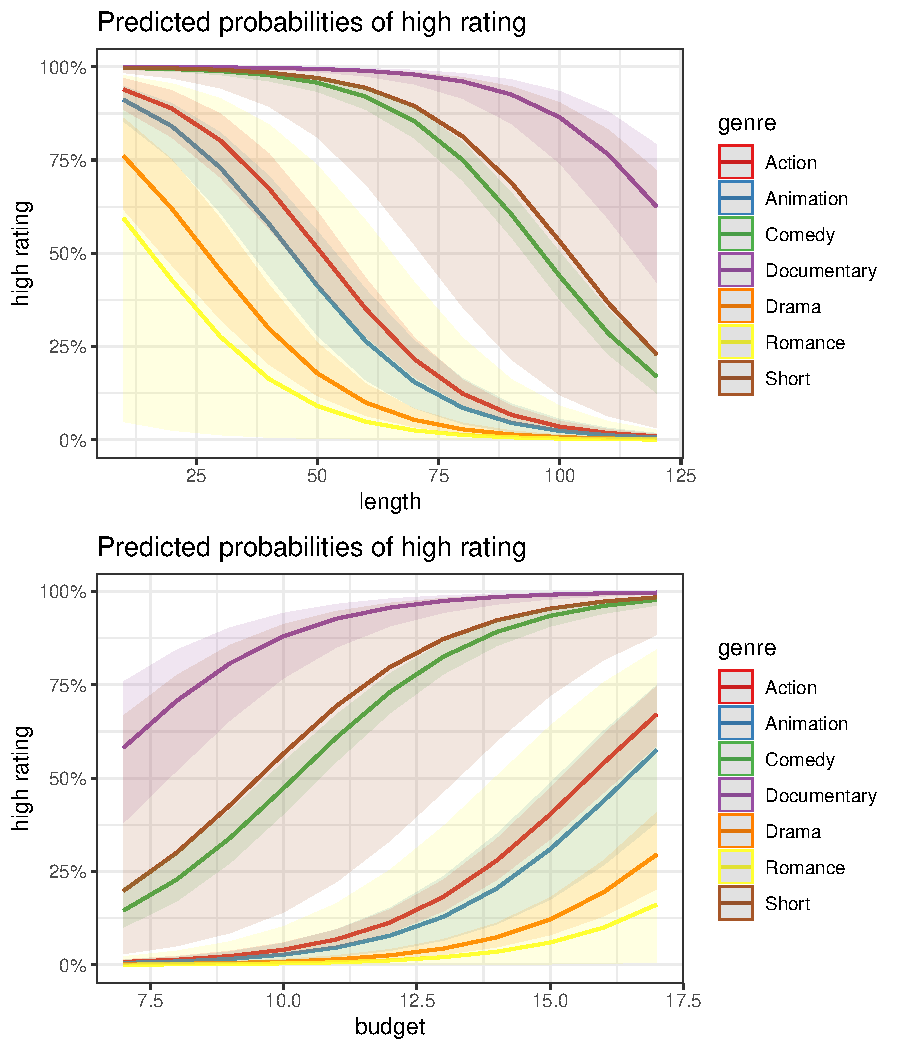
\includegraphics{Group_06_Analysis_files/figure-pdf/fig-probabilities-plot-1.pdf}

}

\caption{\label{fig-probabilities-plot}Plot for Predicted Probabilties}

\end{figure}

\clearpage

The Figure~\ref{fig-probabilities-plot} shows that the probability of a
film to have `Rating greater than 7' increases with the decrease in
length of the film and increases with the increase in budget of the film
for all the genres.

Let's have a look at the first five rows of the new data frame.

\hypertarget{tbl-dataset-final}{}
\begin{longtable}{rrrrrcrccrrrr}
\caption{\label{tbl-dataset-final}Glimpse of the first five rows in the IMDB data set with log-odds, odds
and probabilities }\tabularnewline

\toprule
film\_id & year & length & budget & votes & genre & rating & high\_rating & rate & log\_votes & logodds.m2 & odds.m2 & probs.m2 \\ 
\midrule\addlinespace[2.5pt]
31804 & 2002 & 18 & 9.6 & 15 & Drama & 8.0 & 1 & Rating greater than 7 & 2.708050 & -0.7179778 & 0.487737561 & 0.32783844 \\ 
25453 & 2000 & 98 & 13.8 & 23 & Action & 3.3 & 0 & Rating less than 7 & 3.135494 & -2.1806423 & 0.112968952 & 0.10150234 \\ 
5479 & 1989 & 81 & 11.5 & 57 & Documentary & 7.9 & 1 & Rating greater than 7 & 4.043051 & 2.8412760 & 17.137620048 & 0.94486597 \\ 
44235 & 1995 & 100 & 7.5 & 32 & Action & 3.4 & 0 & Rating less than 7 & 3.465736 & -5.8055102 & 0.003010918 & 0.00300188 \\ 
14580 & 2003 & 80 & 10.8 & 30 & Action & 2.6 & 0 & Rating less than 7 & 3.401197 & -2.6337262 & 0.071810384 & 0.06699915 \\ 
\bottomrule
\end{longtable}

\hypertarget{model-checking-and-diagnostics-sec-mcd}{%
\subsection{Model Checking and Diagnostics
(\#Sec-mcd)}\label{model-checking-and-diagnostics-sec-mcd}}

\hypertarget{Sec-ms}{%
\subsubsection{Model Selection}\label{Sec-ms}}

\begin{enumerate}
\def\labelenumi{\arabic{enumi}.}
\tightlist
\item
  Likelihood Ratio Chi-Squared Statistic Test
\end{enumerate}

\begin{Shaded}
\begin{Highlighting}[]
\CommentTok{\# 1. Likelihood Ratio Chi{-}Squared Statistic Test}
\NormalTok{lrt\_1 }\OtherTok{\textless{}{-}} \FunctionTok{anova}\NormalTok{(m0\_model, m1\_model, }\AttributeTok{test=}\StringTok{"Chisq"}\NormalTok{)}
\CommentTok{\# since p{-}value \textgreater{}0.05 therefore m1\_model better than m0\_model but m0\_model is better than m2\_model}
\NormalTok{lrt\_2 }\OtherTok{\textless{}{-}} \FunctionTok{anova}\NormalTok{(m1\_model, m2\_model, }\AttributeTok{test=}\StringTok{"Chisq"}\NormalTok{) }\CommentTok{\# \# since p{-}value \textless{} 0.05 therefore m1\_model better than m2\_model}
\end{Highlighting}
\end{Shaded}

This test suggests that m1\_model could the best choice based on
Likelihood ration test. However, m0\_model has insignificant term
`log\_votes' and smallest reduction in residual deviance when adding
`year' and `log\_votes'. A model without `year' and `log\_votes' would
be more suitable.

\begin{enumerate}
\def\labelenumi{\arabic{enumi}.}
\setcounter{enumi}{1}
\tightlist
\item
  Residuals
\end{enumerate}

\begin{figure}

{\centering 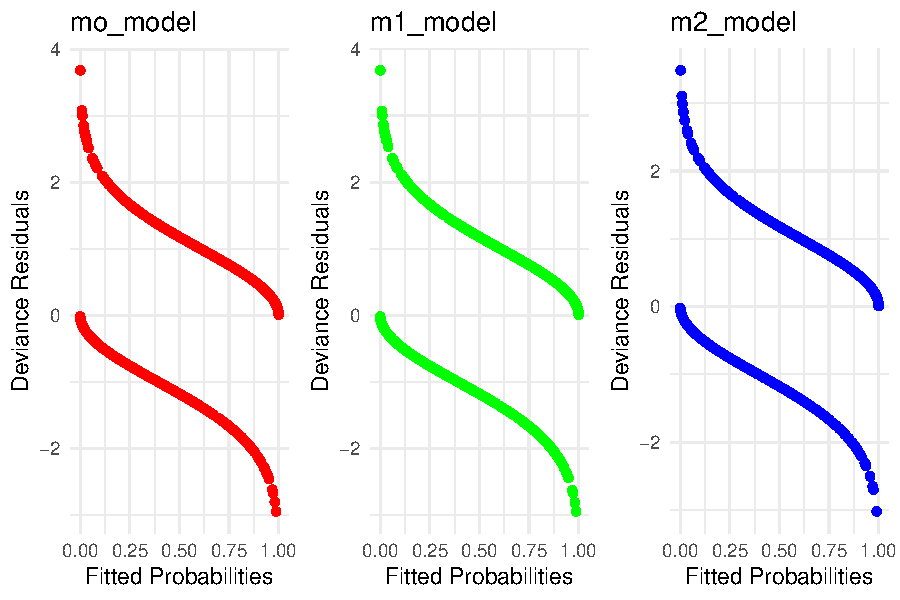
\includegraphics{Group_06_Analysis_files/figure-pdf/fig-residuals-1.pdf}

}

\caption{\label{fig-residuals}Plot for Residuals}

\end{figure}

\clearpage

\hypertarget{tbl-comparison-of-models}{}
\begin{longtable}{lrrr}
\caption{\label{tbl-comparison-of-models}Comparison of Models }\tabularnewline

\caption*{
{\large Model Comparison Table}
} \\ 
\toprule
Model & Mean\_Deviance\_Residual & Mean\_Pearson\_Residual & Mean\_Fitted\_Probabilities \\ 
\midrule\addlinespace[2.5pt]
m0\_model & -0.04961650 & -0.006920083 & 0.3324729 \\ 
m1\_model & -0.04945432 & -0.006295522 & 0.3324729 \\ 
m2\_model & -0.05060707 & -0.009906284 & 0.3324729 \\ 
\bottomrule
\end{longtable}

A comparison of the \ul{Mean Deviance Residual (MDR)} all of the models
fit the data well, with small difference suggesting \textbf{m2\_model}
is a better fit.

\ul{Mean Pearson Residual (MPR)} varies slightly among the three models,
with m0\_model and m1\_model having closer mean values and m2\_model
having the lowest mean value (-0.0099), suggesting that the
\textbf{m2\_model} is a better fit than the the other two models.

The mean value of \ul{Mean Fitted Probabilities} (0.332) is same across
all models, suggesting that the average prediction probability of a film
receiving `Rating greater than 7' is consistent across models.\clearpage

\begin{enumerate}
\def\labelenumi{\arabic{enumi}.}
\setcounter{enumi}{2}
\tightlist
\item
  ROC curve and AUC
\end{enumerate}

\ul{Comparison of ROC curves}, it can be observed from the figure that
the ROC curves of the three models are very close to each other, almost
overlapping, and all three curves are very tightly fitted to the upper
left corner, indicating that all three models have good predictive
ability This suggests that in terms of the balance between the
sensitivity (true rate) and the specificity (false positive rate), these
models have similar classification ability. This is also confirmed by
the AUC values of the models, with m0\_model having the highest AUC
(9,951897), but the differences with m1\_model (0.9518471) and m2\_model
(0.9512016 ) are very slight.

\begin{figure}

{\centering 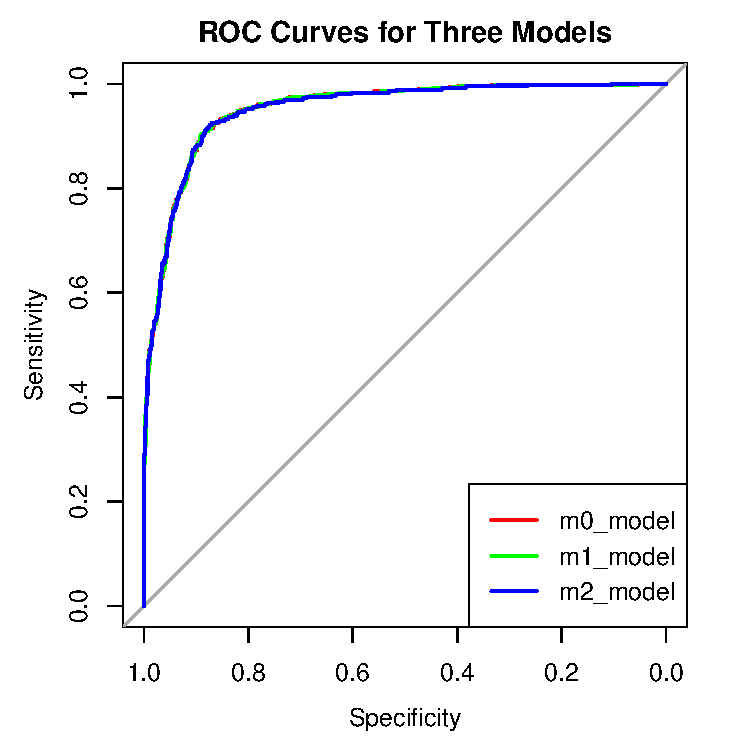
\includegraphics{Group_06_Analysis_files/figure-pdf/fig-ROC-AUC-1.pdf}

}

\caption{\label{fig-ROC-AUC}Plot for Predicted Probabilties}

\end{figure}

\clearpage

\hypertarget{tbl-auc}{}
\begin{longtable}{lr}
\caption{\label{tbl-auc}AUC values }\tabularnewline

\toprule
Model & AUC \\ 
\midrule\addlinespace[2.5pt]
m0\_model & 0.9519078 \\ 
m1\_model & 0.9518664 \\ 
m2\_model & 0.9512197 \\ 
\bottomrule
\end{longtable}

\ul{Comparison of AUC values} shows that all models have very high
predictive performance, with AUC values most 0.95, implying that the
models work well in distinguishing between `Rating greater than 7' and
`Rating less than 7' films. m0\_model shows the best performance, but
the difference with m1\_model and m2\_model is negligible, suggesting
that there is little or no loss in prediction.

4. \textbf{AIC \& BIC}

\hypertarget{tbl-AIC}{}
\begin{longtable}{lrr}
\caption{\label{tbl-AIC}AIC of Models }\tabularnewline

\toprule
Model & df & AIC \\ 
\midrule\addlinespace[2.5pt]
m0\_model & 11 & 1039.973 \\ 
m1\_model & 10 & 1038.067 \\ 
m2\_model & 9 & 1043.170 \\ 
\bottomrule
\end{longtable}

Based on the AIC criterion for model selection, \textbf{m1\_model} (with
log\_votes removed) provided the best fit to the data (AIC = 1038.203)
compared to m0\_model with all variables included (AIC = 1040.110).
Therefore, m1\_model is the preferred model.

\hypertarget{tbl-BIC}{}
\begin{longtable}{lrr}
\caption{\label{tbl-BIC}BIC of Models }\tabularnewline

\toprule
Model & df & BIC \\ 
\midrule\addlinespace[2.5pt]
m0\_model & 11 & 1101.231 \\ 
m1\_model & 10 & 1093.756 \\ 
m2\_model & 9 & 1093.290 \\ 
\bottomrule
\end{longtable}

According to the BIC criterion, the m0\_model shows the highest BIC
value (1101.368), suggesting that this model may not be the most
preferred choice. \textbf{m2\_model} has a lowest BIC (BIC = 1093.426),
suggesting that it is a better choice in a statistical perspective.

\hypertarget{sec-Conc}{%
\section{Conclusions}\label{sec-Conc}}

In comparison to the other models, m2\_model has the minimum BIC. Since
BIC places a stronger penalty on model complexity than AIC for smaller
data sets, simpler model is chosen. m2\_model also performed slightly
better in residual tests. All the parameters of m2\_model are also
statistically significant.It is also noted that even though m1\_model
performed better in likelihood ration test and AIC, it is not preferred
since it has the variable `year' which has the smallest reduction in
residual deviance when adding to the model.

In summary, it can be observed that `length', `budget' and `genre' are
the properties of film that influence the IMDB ratings to be greater
than 7 on not.

\hypertarget{limitations}{%
\subsubsection{Limitations}\label{limitations}}

There are few limitations to the analysis:

\begin{itemize}
\item
  Sensitivity to outliers
\item
  Risk of overfitting the data
\item
  Residuals may not be informative if the response is binary and if
  n\textsubscript{k} is small for most covariate patterns
\item
  The power of the Hosmer-Lemeshow test can be too small to detect lack
  of fit.
\end{itemize}



\end{document}
